
%        File: WeeklyResearchReport_4_19_21.tex
%     Created: Mon Apr 19 08:00 AM 2021 E
% Last Change: Mon Apr 19 08:00 AM 2021 E
%
\documentclass[a4paper]{article}
\usepackage{mathtools}
\usepackage{verbatim}
\usepackage{graphicx}
\usepackage{tabularx}
\usepackage{pgfplots}
\usepackage{adjustbox}
\usepackage{booktabs}
\makeatletter
\let\latex@xfloat=\@xfloat
\def\@xfloat #1[#2]{%
    \latex@xfloat #1[#2]%
    \def\baselinestretch{1}
    \@normalsize\normalsize
    \normalsize
}
\makeatother
\usepackage{amsmath}
\usepackage{mathtools}
\usepackage{epigraph}
\usepackage{cancel}
\usepackage{xcolor}
\newcommand\Ccancel[2][black]{\renewcommand\CancelColor{\color{#1}}\cancel{#2}}
\usepackage{algorithm}
\usepackage{graphicx}
\usepackage[noend]{algpseudocode}
\usepackage{gnuplot-lua-tikz}
\usepackage[utf8]{inputenc}
\usepackage{pgfplots}
\usepackage{tabularx}
\DeclareUnicodeCharacter{2212}{−}
\usepgfplotslibrary{groupplots,dateplot}
\usetikzlibrary{patterns,shapes.arrows}
\pgfplotsset{compat=newest}
\begin{document}
\begin{titlepage}

    \title{
    Daily Research Report}

    \author{ Jeffrey Severino \\
        University of Toledo \\
        Toledo, OH  43606 \\
    email: jseveri@rockets.utoledo.edu}


    \maketitle

\end{titlepage}
\section{Current Research Direction}
Finish running all the cases needed from SWIRL by the 14th

\section{Research Performed}
The MMS plots shown below are a draft idea of how I want to present the data.
I have only presented three grids at very coarse grids to see how certain 
comparisons show differences. The results below are for second order radial 
derivatives.

 \begin{figure}
     \centering
     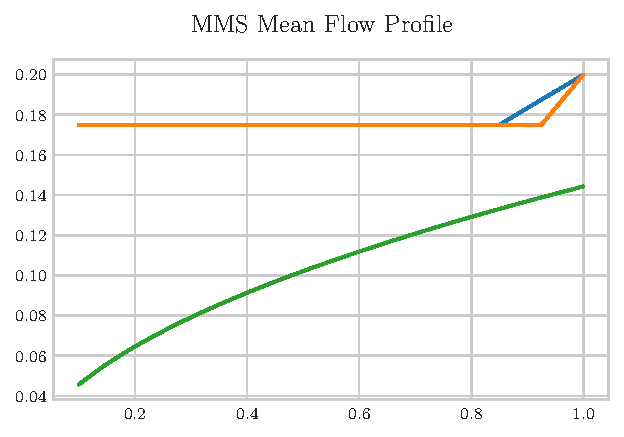
\includegraphics[width=\textwidth]{/home/jeff-severino/SWIRL/CodeRun/03-plotReport/tex-outputs/MMS_meanFlow.pdf}
 \end{figure}



 \begin{figure}
     \centering
     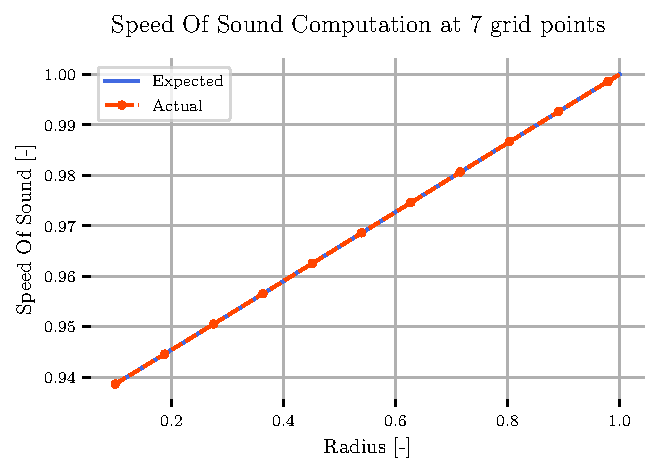
\includegraphics[width=\textwidth]{/home/jeff-severino/SWIRL/CodeRun/03-plotReport/tex-outputs/SpeedOfSoundComparison1.pdf}
 \end{figure}

 \begin{figure}
     \centering
     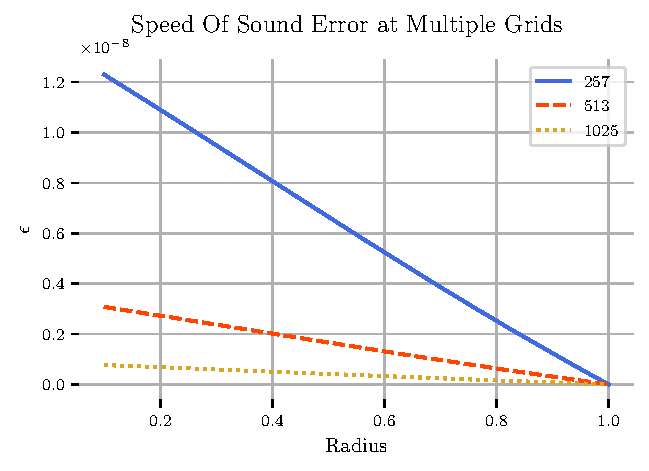
\includegraphics[width=\textwidth]{/home/jeff-severino/SWIRL/CodeRun/03-plotReport/tex-outputs/SpeedOfSoundComparison2.pdf}
 \end{figure}


 \begin{figure}
     \centering
     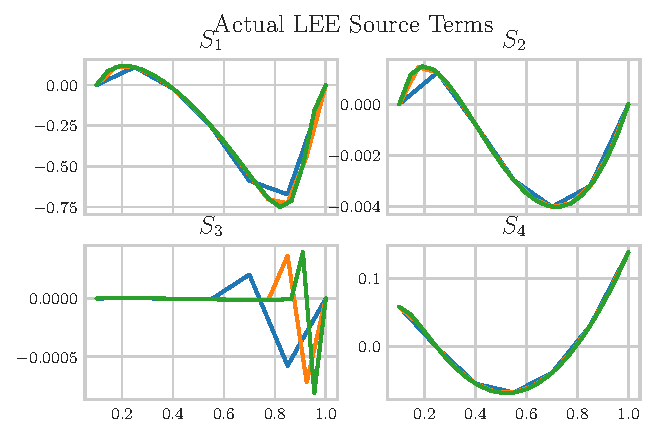
\includegraphics[width=\textwidth]{/home/jeff-severino/SWIRL/CodeRun/03-plotReport/tex-outputs/SourceTermActual.pdf}
 \end{figure}

 \begin{figure}
     \centering
     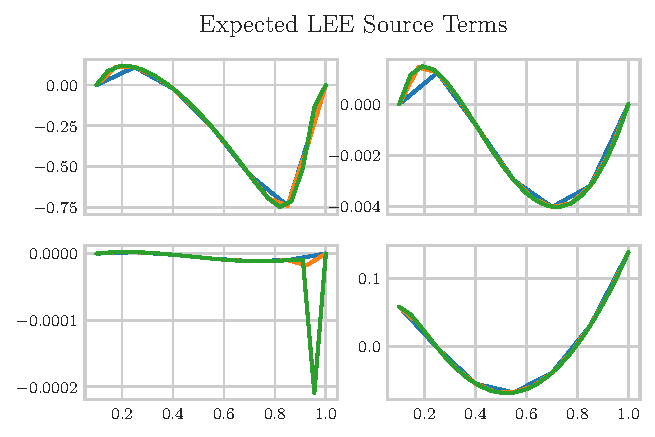
\includegraphics[width=\textwidth]{/home/jeff-severino/SWIRL/CodeRun/03-plotReport/tex-outputs/SourceTermExpected.pdf}
 \end{figure}


 \begin{figure}
     \centering
     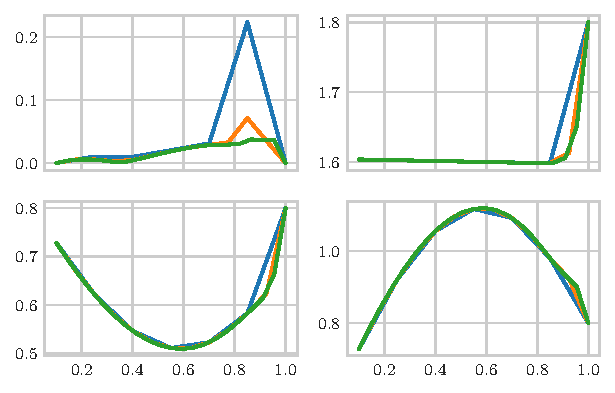
\includegraphics[width=\textwidth]{/home/jeff-severino/SWIRL/CodeRun/03-plotReport/tex-outputs/SourceTermError.pdf}
 \end{figure}




\section{Issues and Concerns}
How do I report code timing? 

I need to put a user warning about potential conflicts in the MMS just in case.
\section{Planned Research}
Get plots for fourth order approximations. Require only one run for both second 
and fourth.
Add accompanying functions for

\begin{enumerate}
    \item MMS mean flow 
\end{enumerate}
Mean flow 

\end{document}


